\documentclass[a4paper,11pt]{article}

\usepackage[latin1]{inputenc} % pour les accents
\usepackage[T1]{fontenc}
\usepackage[francais]{babel}
\usepackage{fullpage}
\usepackage{color}
\usepackage{amsmath}
\usepackage{url} 
\usepackage{makeidx}
\usepackage{amsmath}
\usepackage{wasysym}
\usepackage{float}
\usepackage{graphicx}
\usepackage{a4wide}
\usepackage{multirow}
\usepackage{afterpage}
\usepackage{pst-all} % Pour pstricks
\usepackage{moreverb}

\definecolor{gray}{gray}{0.85}

\title{
  \normalsize{\begin{flushright} MASTER 2 - Semestre 1 - 2008 \end{flushright}}
  \vspace{15mm}
  \hrule height 1mm
  \vspace{5mm}
  \Huge{\emph{Qualit� et fiabilit� logicielle\\\textsl{Puissance 4} en Java et
      tests logiciels}}
  \vspace{5mm}\hrule height 1mm
  \vspace{1cm}
}

\author{
  MALEVILLE Nicolas\\
  LAMARTI Abdessamad\\
  DUBERNET Jean S�bastien\\
  CRANSAC Dorian\\
  EWANS Edouard\\
  SELLIER Xavier
  \vspace{2cm}
}

\date{}

\begin{document}
\begin{titlepage}
  \begin{figure}
    \vspace{1cm}
    \psset{unit=1in,linewidth=4pt} %param�trage des unit�s pour pstricks
    \rput(1,0){
\includegraphics[width=4cm]{Bordeaux1}}
    \vspace{15mm}
  \end{figure}
\end{titlepage}

\maketitle

\vspace{4cm}
\begin{center}
Enseignant : Rollet
\end{center}

\newpage
% -*- mode: latex; coding: latin-1-unix -*- %

\section{Introduction}

Il y a pas mal de choses � revoir et il faut se mettre d'accord.


\newpage
% -*- mode: latex; coding: latin-1-unix -*- %

\section{Besoins fonctionnels}

\begin{itemize}
 \item \texttt{grille 6 lignes * 7 colonnes}
 \item \texttt{Aggrandir (partie no ngraphique)}
 \item \texttt{Player vs Player}
 \item \texttt{Player vs Computer}
 \item \texttt{Computer vs Computer}
 \item \texttt{Strat�gie gagnante}
 \item \texttt{2 niveaux d'IA}
 \item \texttt{conditions de fins de jeux}
 \item \texttt{Modularit�}
 \item \texttt{Affichage mode texte (par d�faut)}
\end{itemize}
\section{Besoins non-fonctionnels}

\begin{itemize}
 \item \texttt{r�activit�}
 \item \texttt{barre de progression / t�moin d'avancement}
\end{itemize}


\newpage
% -*- mode: latex; coding: latin-1-unix -*- %

\section{Diagramme}

On  stocke notre structure de donn�es dans une matrice (pour le moment
... a revoir).

\begin{figure}[!h]
\begin{center}
  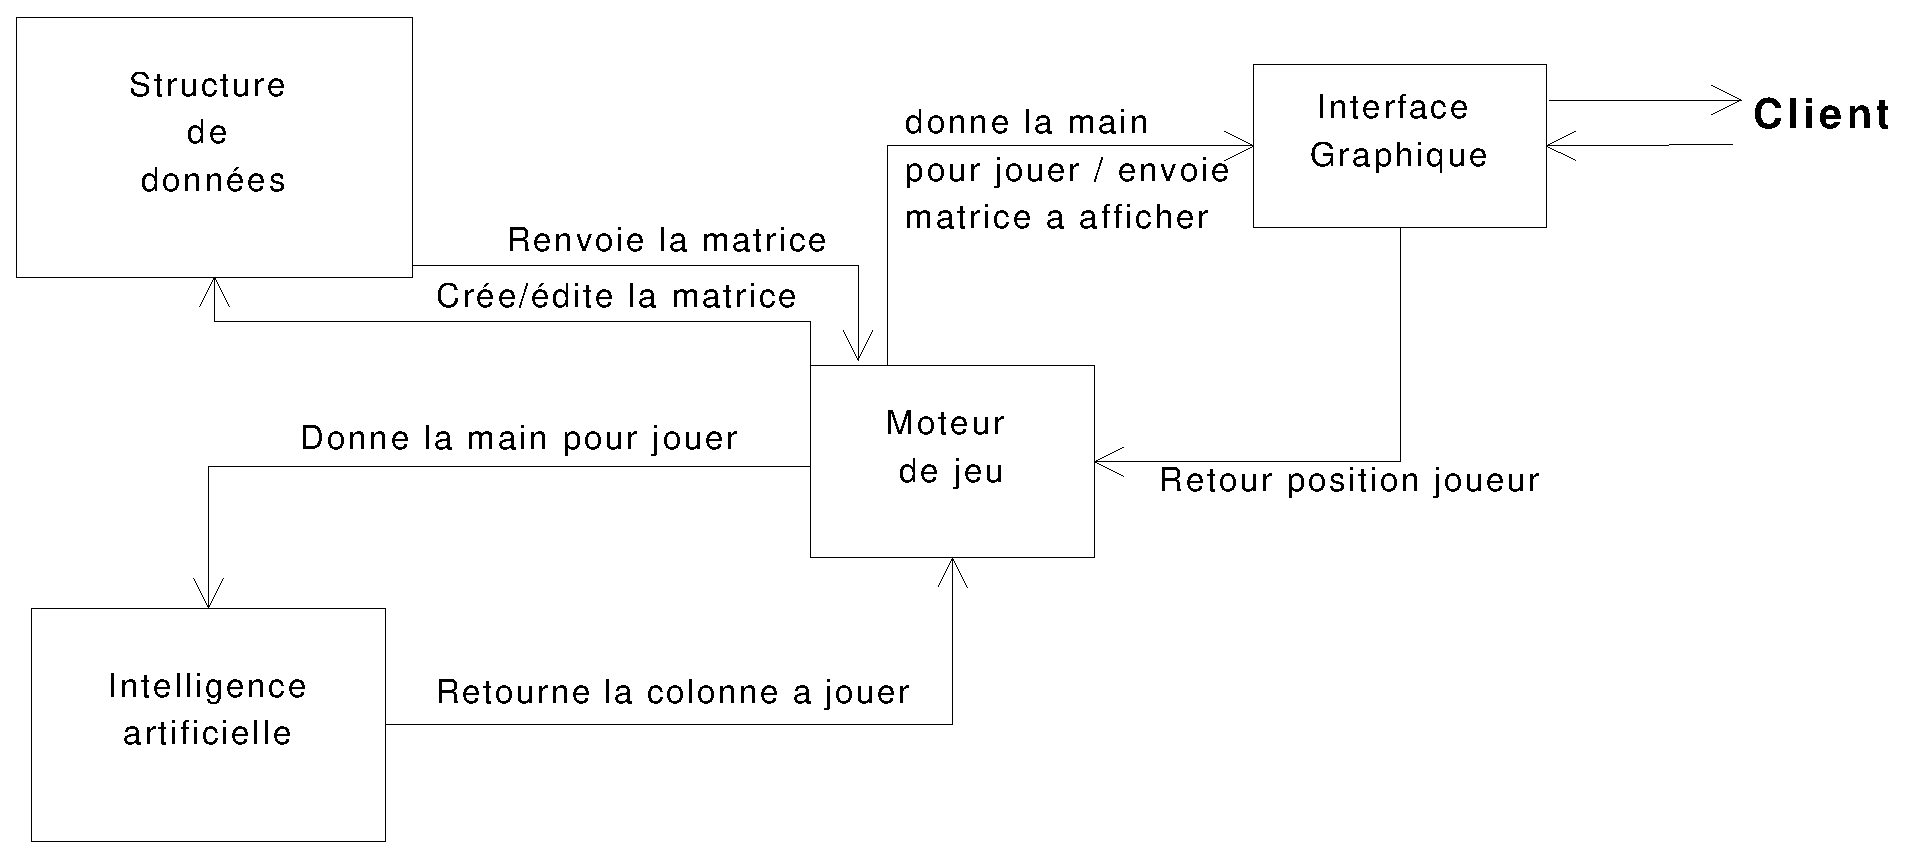
\includegraphics[scale = 0.5]{diagramme}
  \caption{Diagramme de fonctionnement}
  \label{diagramme}
\end{center}
\end{figure}


\newpage
% -*- mode: latex; coding: latin-1-unix -*- %

\section{Prototype}

Une liste des prototypes des fonctions :

\subsection{Structure de donn�es}

\begin{itemize}
 \item \textsl{create\_matrix(int width, int height, int color);} -
   cr�e notre matrice
 \item \textsl{get\_matrix();} - retourne notre matrice
 \item \textsl{set\_matrix(int i, int j, int color);} - modifie une
   case de notre matrice
\end{itemize}

\subsection{Moteur de jeu}

\begin{itemize}
 \item \textsl{constructeur(int nb\_joueur);} - notre constructeur de
   taille 6 * 8 de base
 \item \textsl{constructeur(int nb\_joueur, int width, int height);}
   - notre constructeur de taille minimale 6 * 8
 \item \textsl{get\_grid();} - retourne notre matrice
 \item \textsl{add\_jeton(int i, int j, int color);} - ajouter un
   jeton au joueur correpondant
 \item \textsl{gravity(int i, matrix grid);} - retourne la hauteur de
   la case libre � la colonne i.
 \item \textsl{statement();} - notre �tat courant
 \item \textsl{check\_victory(matrix grid);} - v�rifie si il quelqu'un
   a gagn�
\end{itemize}

\subsection{Interface Graphique}

\begin{itemize}
 \item \textsl{print\_grid(matrix grid);} - Affiche la grille
 \item \textsl{play(int id\_player);} - Attend une action du joueur
\end{itemize}


\end{document}
